\chapter{Карта и описание местности}

\begin{center}
\includegraphics[width=\linewidth]{chast-zmiy/karta-opis/smor-map-2014.pdf}
\end{center}

Эта карта отражает состояние местности на 2014 год.

Легенда карты такова:

Серым цветом отмечена промзона. Промзона к северо-востоку от улицы Кирилловской лежит на низменной Оболони. В отдалении около – в разные века по-разному, но примем два километра – параллельно улице, протекала Почайна. К востоку от Богуславского спуска промзона расположена на равнине и несколько заползая на склон.

Коричневым цветом обозначена жилая застройка.

Светло-зеленым цветом отмечена местность, так или иначе заросшая лиственным лесом. Почти вся она находится на возвышенности Кирилловских высот.

Синий прямоугольник показывает примерно окрестности бывшей усадьбы Светославского. Я не знаю ее границ.

Голубая пунктирная линия – ручей в овраге близ усадьбы Светославского.

Крест – церковь Николая Чудотворца «Памяти жертв Чернобыля».

Малиновый прямоугольник – мемориал жертвам Чернобыльской катастрофы, с современным курганом.

Фиолетовый прямоугольник – бугристая местность, покрытая рощей. 

Желтоватый пунктир – грунтовка вдоль возводящихся коттеджей, она же – остаток прежней ветви Смородинского спуска.

Оранжевый кружочек – раскопанный суглинный склон, в том месте немного возвышающийся над дорогой.

Синий кружочек – совсем маленькая пещерка на обрывистом склоне.

Зеленый кружок – две пещеры в уже довольно крутом и высоком склоне над дорогой. Называю их Левой и Правой Малыми пещерами. Примерные координаты – 50°28'39.19"N 30°28'38.92"E.

Красный кружок – Кирилловская пещера, Логово Змия. Склон в том месте сильно возвышается над дорогой, пещера – ближе к его верху, вход в нескольких метрах от поверхности плато. Координаты приблизительно 50°28'41.03"N 30°28'46.32"E. 

Чтобы лучше понять настоящее, надо основательно изучить прошлое. И рассмотреть местность в связи с окрестностями, не попавшими на карту или затронутыми частично.

Итак, нарисованный «зеленый» массив более или менее отражает очертания средней части Кирилловских высот, поднимающихся над плоской Оболонью. Раньше, идя от них прочь на восток, мы бы вышли по лугам к Почайне.

Сейчас все отроги Кирилловских высот покрыты лиственным лесом. А в 1940-х, например, отрог Смородинского спуска был голым, только трава росла.

На западе крупной дорогой нисходит к Кирилловской выложенный темной брусчаткой Подольский спуск, в одном месте приблизившись к Смородинскому на 30 метров. Кирилловская и смежная с нею пещеры находятся на другом отроге, нежели Подольский спуск. Оба спуска, Подольский и Смородинский, разделены оврагом, начинающемся на уровне западной стороны того резкого колена, которое Смородинский выкидывает в месте приближения к Подольскому.

Подольского спуска раньше не было. Его проложили в середине 1950-х. При этом изменения в местности произошли следующие. 

Уничтожили верхнюю часть Смородинского спуска. Перед курганом мемориала жертв Чернобыля, на запад шла улица, отрезок Смородинского спуска – исчезла. В западной части прервали улицу Нагорную, что прежде продолжалась и соединялась с Пугачева, откуда свернувший с Овручской по Нагорной трамвайный маршрут нырял в нынешний Врубелевский спуск – улочку в Репяховом яру, что отделяет мыс Подольского спуска от горы с Кирилловской церковью.

На Куренёвку, к стадиону «Спартак» (под горой с Кирилловской церковью), спуститься можно было тремя способами. По Репяховому яру на трамвае. Узенькой Макаровской улицей, вдоль Репяхового яра гребнем холма. Смородинским спуском.

Во время прокладки Подольский спуск захватил низовья Макаровской и Репяхового яра, ручей в котором взяли в коллектор, а мостик над ручьем уничтожили. 

Главное колено Смородинского спуска начиналось южнее нынешнего –  от кургана (коего тогда не было), в целом же спуск повторял современные очертания, но с поправкой. В юго-восточном углу прежних очертаний колена, на северо-восток отделялась грунтовка. Сейчас по ее месту два отрезка. Один мощенный брусчаткой, от церкви и вниз до первого поворота. А дальше теперь вдоль особняков идет грунтовка. Справа дом\'а, слева – склон с пещерами. Грунтовка еще в пятидесятых доходила к северному склону, над улицей Кирилловской, и резко сворачивала там на запад к основной дороге Смородинского спуска. Поворот сохранился поныне, примыкая к нижней части спуска.

Прежнее колено было гораздо больше нынешнего и западной частью лежало на современном восточном склоне горы вдоль Подольского спуска. Этот спуск насквозь пробил Нагорную и Смородинский спуск, первую обрубив рукотворным оврагом, а у второго сократив петлю колена там, где теперь Смородинский и Подольский спуски сближаются. Раньше, петля Смородинского соседствовала через пустырь с Макаровской улицей.

Поглядим на аэрофотоснимок 1943 года.

\begin{center}
\includegraphics[width=0.80\linewidth]{chast-zmiy/karta-opis/obsh-map.jpg}
\end{center}

Главный ориентир – стадион «Спартак» в верхнем левом углу иллюстрации, и длинная прямая улица в левой части – это Макаровская. Наискосок всего кадра проходит улица Кирилловская. В нижнем правом углу виден мыс Кирилловской стоянки. Точно в середине изображения – мыс с Кирилловской пещерой, его западная граница темнеет эдаким треугольником.

На советской топографической карте тоже нет еще Подольского спуска и хорошо расписаны высоты.

\begin{center}
\includegraphics[width=0.80\linewidth]{chast-zmiy/karta-opis/sov-map.jpg}
\end{center}

 По всем закоулкам мы еще пройдем, в свое время, пока же сосредоточимся на Смородинском спуске.

Когда он возник как поименованный? Понятное дело, что овраг существовал и раньше, а вот название должен был получить, когда им стали пользоваться. Для спуска ли по нему, или житья в окрестностях. Рогович в 1876 году называл тамошний яр оврагом Балашова, а всю местность Загоровщиной. На 1870 год на карте обозначена «земля дочери майора Елизаветы Балаш». В то же время лежащий через водораздел Репяхов яр отмечен, под именем Кирилловского оврага, как владение Багговута.

Разберем старые карты. В первой половине 19 века на месте Смородинского спуска – дикая гора с узнаваемым яром. Чтобы добраться на Куренёвку, варианта два – по дороге от Подола вдоль Кирилловских высот (прообраз улицы Кирилловской), а если сверху от Лукьяновки – то через овраги около Иорданской церкви, либо по современной Макаровской. Тогда это была просто грунтовая дорога. Однако жилые домики уже стояли и у нижней части будущего Смородинского спуска.

В конце 19 века Смородинского спуска еще нет. Местность его и окрестностей на картах того времени подписана как «Дачи». Внизу, к северо-западу от начала будущего спуска, на месте нынешнего сквера около домов на Кирилловской 99/1К3, 99/1К2, 99/1К1, короче говоря напротив стадиона через Подольский спуск, возникла Кирилловская площадь с базаром (не путать с Куренёвской площадью и ее толкучкой, Птичьим рынком). Дом Викентия Хвойки (у него было жилье также на Игоревской 9/1) в 1911 году имел адрес Троицко-Кирилл\-овская площадь, 4 (прежнюю Троицкую площадь переименовали в Куренёвскую). Поблизости жил еще Езерский, и когда рядом под прямым углом к Кирилловской проложили новую улицу, поначалу она носила название Езерской, а потом ее переименовали в Викентия Хвойки. На площади был и разворот 18-го трамвая из Репяхового яра.

За сквером\footnote{В 1978 году при археологических раскопках примерно на этом месте, около Кирилловской, 90, нашли два культурных слоя «древнерусского времени» – как считают, 12-13 веков. Один, метровый слой, залегал на глубине 1,5 метра, затем шел песок, и на глубине 5 метров – еще полуметровый культурный слой. В первом были железные гвозди, лезвие ножа, светло-зеленые поливные плитки пола, битый кирпич, прясла, черепки. Обнаружили остатки глинобитной, толстостенной печи с полом, обложенным черепками и кусками кирпича. В печи лежали куски железного шлака или крицы, шлак валялся и рядом. Значит, тут производили из руды железо, а местность была если не частью давнего Киева, то его присёлком.} – несколько жилых домов, закрытая (в 2013 году) школа, еще некое аварийное здание – кажется, в квартале идет сплошной ремонт. Этот уголок, центром которого была Кирилловская площадь, слывет Липлиновкой, по фамилии бывшего землевладельца (психиатр Константин Михайлович Леплинский, его клиника была по адресу Кирилловская, 99). В середине 1930-х на месте площади, хат с палисадниками, огородами и пустырей создали парк с танцплощадкой и стадионом «Спартак». От большого парка теперь остался только сквер (на месте Кирилловской площади) да стадион. 

\begin{center}
\includegraphics[width=\linewidth]{chast-zmiy/karta-opis/\myimgprefix ex-kyr-plosh-2013.jpg}

\textit{2013 год, сквер на месте Кирилловской площади.}
\end{center}

На стадионе поначалу не было трибун – просто поле, пара деревянных домиков и раздевалка. Директором работал одноглазый Слуцкий, выдававший спортсменам инвентарь и форму. После войны наконец построили трибуны, тир, площадки для волейбола, тенниса, баскетбола, памятник Сталину у входа, и четыре гипсовые скульптуры атлетов. Когда именно – не знаю, на снимке 1955 года трибун еще не видно.

До 1950-х, до прорытия Подольского спуска, около стадиона был перекинут мостик через ручей, вытекавший из Репяхового яра. Леонид Коныхов в «Киевских рассказах» пишет:

\begin{quotation}
Сейчас того мостика нет. Будете искать – не найдете. Он исчез вместе с инвалидом, который продавал там самодельные конфеты в деревянном ящике со стеклянной крышкой. Мостик убрали, когда строили дорогу Подольского спуска, правую границу Липлиновки. Это еще хорошо, что Витька Шило перелетел через перила и упал с мостика в ручей, где мягкий песочек под мелкой водой.
\end{quotation}

Когда едешь с Лукьяновки выложенным трясучей, черной брусчаткой Подольским спуском, примерно на половине пути видишь справа, вровень с собой верхушки деревьев и домов – это и есть, под крутым склоном, большая часть Липлиновки. В приближении к перекрестку у стадиона, ниже, по левую руку за зеленью тоже скрывается глубина, там же – Репяхов яр, однако не зная этого, люди мельком примечают только зелень, такую же, как по горе выше, где над спуском громоздится холм со стриженым травянистым боком и рощицей наверху, граничащей с частным сектором по Макаровской.

Напротив юго-восточных зданий Липлиновки, по другую сторону улицы Кирилловской, заканчивается жилой массив и начинается промзона. К востоку от нее раньше, в виду Кирилловских высот, через поле, протекала в давнее время Почайна. Относительное расположение Почайны, цепи холмов и луговой части очень важно, о чем мы поговорим в свое время.

Карта 1911 года на месте Смородинского спуска изображает целый букет улиц! Это Димовский спуск, улица Иполитова и между ними смычка – Мишин переулок.

Снизу, к перекрестку Нагорной и Димовского спуска, присоединяется Овручская улица, как и теперь. Карты 1912-13 годов вместо букета являют пустоту. На карте 1914 года нарисована, без подписи, продолжением Овручской некая дорога с «коленом» в пределах Смородинского спуска, однако слишком прямоугольная, чтобы быть правдой.

\begin{center}
\includegraphics[width=\linewidth]{chast-zmiy/karta-opis/1911-smor-map-pal.png}

\textit{Фрагмент карты 1911 года.}
\end{center}

Затем снова картографическое забвение до 1918 года, где на немецком плане снова букет – Димовский (Диновский, Димновский?) спуск, улица Иполитова да Мишин переулок. По немецкой-то карте становятся ясными составные части будущего Смородинского спуска в виде, каким он был до прорытия Подольского спуска. Давайте поглядим вместе.

\begin{center}
\includegraphics[width=\linewidth]{chast-zmiy/karta-opis/1918-smor-map.png}

\textit{Фрагмент карты 1918 года.}
\end{center}

Димовский спуск начинался перед местом, где ныне курган, непосредственно к югу от него. Оттуда дорога шла на запад (через разбитый в конце 2016 года сквер) в сторону Макаровской улицы. Затем видим возврат колена на восток и примерное повторение линии современного Смородинского спуска от пересечения с Мишиным переулком и ниже. 

Мишин переулок – это отрезок современного Смородинского спуска между Подольским спуском и восточным поворотом основного колена\footnote{50°28'37.5"N 30°28'46.87"E}. Наконец, улица Иполитова – то, что я именую «грунтовкой» применительно к части старого Смородинского спуска.

\begin{center}
\includegraphics[width=\linewidth]{chast-zmiy/karta-opis/smor-map-1918.pdf}
\end{center}

Отмечу на основной карте линиями:

Зеленая линия – Димовский спуск.

Фиолетовая линия – Мишин переулок.

Красная линия – улица Иполитова.

На картах 1920-х годов эти улицы подписаны частично, на карте 1930-го вместо Димовского спуска явлен миру Дюковский, Мишин переулок переделывается в Мышин, а улица Иполитова теряет название, хотя обозначена. Спустя год Иполитова появляется то ли как спуск, то ли как переулок – «Іпполітівський». 

Уже в 1932 году на схеме «маршрутов и проездов» вместо этих улочек и спусков обозначен, по контуру Смородинского спуска 2014 года, но с прежним большим «коленом», «Смородиновий узвіз», выходя внизу точнехонько на Асбесто-шиферный завод. В справочниках любят писать, что спуск назвали так по старинной фамилии купцов Смородиновых. Как мы видим, переименование произошло в тридцатые годы, когда про купцов вряд ли вспомнили бы – скорее, это могла быть фамилия местного или отдаленного партийного деятеля. Также не выдерживают проверки сведения о речке Смородине.

Карта 1935 года, теперь это «Смородинський узвіз», но сохраняются переулок «Мышив» и переулок Иполитовский. На немецкой карте 1941 года есть Смородинский спуск да Иполитовский переулок. Судя по уже советской карте 1943 года, на южной части «колена», по обе стороны (то есть на отрезке, что шел мимо нынешнего кургана) было несколько зданий – два по северной стороне, три по южной. Остальная часть спуска и Мишин переулок – пусты. Здания виднеются только внизу, в районе Липлиновки вдоль улицы Кирилловской. Немцы не унимались и в 1943 году составили свою карту. Там показан Смородинский спуск – по бывшему Димовскому и по Иполитовской улице. Отмечен еще «Мышин» переулок. Такая разметка, но без Мышина, принята на отечественной карте за 1947-й. Позже от Смородинского остается только «основная» ветка, что была Димовским спуском, без отрезка от кургана до нынешнего Подольского спуска. На многих советских картах Смородинского спуска вообще нет.

Так сохранялся уголок древности, пока в 21 веке к нему не добрались вездесущие строители. Как долго продержится Смородинский спуск – неведомо. Уже трещит по швам. Поэтому важно сохранить память о нем хотя бы в книге.

Совершим прогулку, не заходя пока в пещеры. Туда мы полезем позже. Просто запечатлеем местность, как она есть в году 2014. Теперь, когда мы знаем составляющие Смородинского спуска – Димовский спуск (в варианте с урезанным коленом), Мишин переулок, Иполитовскую улицу – будет проще давать ориентиры, описывать, как к чему пройти. Вместо нелепых указаний свернуть на таком-то повороте, я просто скажу – от Мишиного переулка туда-то. 

Пещеры можно посетить, двигаясь снизу или сверху спуска. Путешествие снизу позволяет лучше погрузиться в древнее, мрачное и сказочное настроение Смородинского, зато по верху легче и быстрее! Я опишу оба пути, что позволит осмотреть верхнюю и нижнюю половины спуска.

Начнем сверху. Сюда мы доберемся от станции метро Лукьяновская пешком – полчаса ходьбы. Улицей Мельникова, затем свернем и по Герцена, вдоль парка Котляревского на улицу Овручскую. 

%Тут кстати уцелел старинный одноэтажный дом под номером 5, а в его переулке – замечательные граффити, сюжетно связанные с мультфильмом «За 80 дней вокруг света». Надпись на стене дома гласит: «Используй всё что под рукою, и не ищи себе другое».

А на другой стороне, за оградой бывшей, как в народе говорят, дачи Хрущева, в темном яру сочится из склона один из двух истоков Глубочицы – и через каскад замусоренных прудов исчезает в коллекторе. Это место – маленький тенистый парк на территории Института педиатрии, акушерства и гинекологии, мы показали в фильме «Киевская сюита». 

%\newpage

%\begin{center}
%\includegraphics[width=\linewidth]{zmiy/IMG_20130604_152101.jpg}
%\end{center}

%\begin{center}
%\includegraphics[width=\linewidth]{zmiy/IMG_20130604_151818.jpg}
%\end{center}

%\newpage

По Овручской нам идти к Нагорной, однако путь  пересекает Багговутовская. Слева, в бывшем сквере, обнесенные забором раскопки и попытки возродить церковь святого Феодора, возведенную стараниями Багговута. Здесь же был разворот трамвайного маршрута, что следовал дальше по Овручской к Нагорной, а оттуда пересекая Макаровскую в Репяхов яр и по нему до Кирилловской площади. Чуть далее от Багговутовской Овручская, застроенная там вековой давности зданиями в пару этажей, следует наверх и прямо, а Подольский спуск отделяется влево. 

\begin{center}
\includegraphics[width=0.90\linewidth]{chast-zmiy/karta-opis/\myimgprefix IMG_20130623_155220.jpg}

\textit{2013 год, вид Овручской улицы от Подольского спуска в сторону Багговутовской.}
\end{center}

По Овручской выходим на перекресток с Нагорной, даже эдакую площадь. Тишина, сонное состояние, торговый киоск родом из девяностых. Нависает здоровенная, 1940 года угловая сталинка по адресу Нагорная, 8/32 – так называемый Красный дом.

\begin{center}
\includegraphics[width=\linewidth]{chast-zmiy/karta-opis/\myimgprefix IMG_20130623_154741.jpg}

\textit{Снимок 2013 года.}
\end{center}

С другой стороны площади, над террасе над другой террасой, вплотную друг к другу стоят два старых дома, трехэтажный, 1912 года постройки, номер 5 (бывший доходный дом межевого инженера Владимира Львова, затем коммуналка Кабельного завода) и двухэтажный 7-й, построенный межевым инженером Горбуновым, а затем тоже ставший коммуналкой Кабельного. Второй этаж – деревянный. Если проведать мощеный булыжником закоулок Нагорной в сторону Подольского спуска, на самом краю горки встретим ветхий, низенький домик номер 2. Нагорная длилась и дальше, а теперь обрублена Подольским спуском. Там, где нынче рукотворный овраг, была земля, и по Нагорной к Макаровской шел трамвай в Репяхов яр.

Смородинский спуск, тоже крытый булыжником, начинает сбегать вниз от площади. Здесь он еще в хорошем состоянии. Оно ухудшается после участка стройки коллектора – асфальт сошел кусками, а булыжник сильно раздолбан, местами вывален благодаря воздействию тяжелой строительной техники. Некоторые водители рискуют машинами и пользуются этой дорогой, чтобы объехать Подольский спуск. Сокращение весьма сомнительное. На велосипеде спуск преодолеть трудно, невозможно. Сверху вниз мешает булыжник, а наоборот – крутизна.

У площади, в самом верху спуска, зеленеет скверик, выходящий к церкви Николая Чудотворца «Памяти жертв Чернобыля». По другую сторону от нее – «мемориал жертвам Чернобыльской катастрофы». Это небольшой, но узкий овраг с подвешенным колоколом. Оттуда дорожка к могучему кургану с крестом. Берега оврага, на коих любят отдыхать забредшие сюда люди, тоже напоминают курганы.

\begin{center}
\includegraphics[width=\linewidth]{chast-zmiy/karta-opis/\myimgprefix IMG_20140609_145409.jpg}
\end{center}

Что же тут было раньше? По аэрофотоснимку 1943 года здесь, на террасе с курганом – участок Смородинского спуска, видны некие огражденные участки, пять домов. Потом была ровная площадка, где росли черешни. На месте уже пустыря, между курганом и Подольским спуском, осенью 2016-го проложили дорожки сквера. А ниже к бывшему Мишину переулку, ныне виднеются земляные бугры, подозрительно похожие на остатки настоящих курганов.

%Не будем забывать, что всего в полукилометре на юго-восток отсюда Хвойка таки обозначил на своей карте курганы, примерно на той же высоте, что Мишин переулок. Да и упоминал о курганах в усадьбе Зарембских. Предположение имеет уже несколько оснований – внешний вид местности, и близость к курганам Хвойки. Да и «три могилы» с плана 1752 года припомним. Но именно «мемориальный» курган насыпан уже в наше время – это я узнал от старожила. Прежде там была полянка.

Мемориал служит началом трассы велосипедистов-да\-ун\-хильщиков. Она, через рощу за курганом срезая поворот спуска, выходит в дикую местность и проходит точно над Змиевой, Кирилловской пещерой – а поскольку там устроен трамплин, велосипедисты, не ведая, что творят, каждым веселым своим катаньем обрушивают в пещере потолок и стены.

\vspace*{\fill}

\begin{center}
\includegraphics[width=\linewidth]{chast-zmiy/karta-opis/\myimgprefix IMG_20160330_140002.jpg}

\textit{Вид от кургана в сторону Подольского спуска. Вперед – исчезнувший отрезок Димовского спуска. Справа вниз, вне кадра – Мишин переулок. Слева наверх, через несколько террас – дома 5 и 7.}
\end{center}

\vspace*{\fill}


\newpage
\begin{center}
\includegraphics[width=\linewidth]{chast-zmiy/karta-opis/\myimgprefix IMG_20160330_140047.jpg}
\textit{Вид на западный берег оврага.}
\end{center}

\begin{center}
\includegraphics[width=\linewidth]{chast-zmiy/karta-opis/\myimgprefix IMG_20160330_140050.jpg}
\textit{На восточный берег оврага.}
\end{center}
\newpage

\begin{center}
\includegraphics[width=0.97\linewidth]{chast-zmiy/karta-opis/\myimgprefix IMG_20160330_140327.jpg}

\textit{Вид с Мишина переулка наверх, на юг, к «исчезнувшему отрезку».}
\end{center}

\begin{center}
\includegraphics[width=0.97\linewidth]{chast-zmiy/karta-opis/\myimgprefix IMG_20160330_140350.jpg}

\textit{То же самое.}
\end{center}
\newpage

\begin{center}
\includegraphics[width=0.96\linewidth]{chast-zmiy/karta-opis/\myimgprefix IMG_20160330_140418.jpg}

\textit{Там же, видна терраса. На карте 1937-го, домик, некое строение было выше террасы.}
\end{center}


\begin{center}
\includegraphics[width=0.96\linewidth]{chast-zmiy/karta-opis/\myimgprefix IMG_20160330_140438.jpg}

\textit{Вид с восточного конца Мишиного переулка на северо-запад, заметен Подольский спуск.}
\end{center}

\newpage
\begin{center}
\includegraphics[width=0.99\linewidth]{chast-zmiy/karta-opis/\myimgprefix IMG_20160330_140510.jpg}

\textit{Вид с той же точки на юг.}
\end{center}

\begin{center}
\includegraphics[width=0.99\linewidth]{chast-zmiy/karta-opis/\myimgprefix IMG_20160330_140546.jpg}

\textit{Вид от колена Смородинского спуска (конец Мишиного переулка) вблизи Подольского спуска, на юг.}
\end{center}

\newpage

Вижу необходимость описывать и показывать всё подробно, ибо не знаю, что уцелеет через несколько лет. В 2016 году в окрестностях Смородинского спуска то началась очередная стройка, то сами окрестности вознамерились превратить в ландшафтный парк для народного удовольствия. Поэтому упорно держусь года 2014 (хотя предыдущая череда снимков относится к весне 2016) и продолжаю повествование.

В этих-то коричневых, поросших деревьями пустырях над Мишиным переулком мне и видятся следы давних курганов, какие-то ровные проходы в земле, не говоря уже о четко сохранившихся террасах.

Ниже церкви, Смородинский спуск, понижаясь, описывает полукруг, включающий в себя Мишин переулок. Поначалу справа возникаю особняки за кирпичными оградами, а напротив них, к западу от кургана темнеет чаща – здесь вглубь некогда уходило начало большого «колена» Димовского спуска. Но мы следуем прямо (на северо-восток), по началу прежней Иполитовской улицы, между продолжением коттеджей и рощей.

Там, где начало (восточное) Мишиного переулка, Смородинский спуск поворачивает к западу. Прямо же, на северо-восток, идет грунтовка (бывшее продолжение Иполитовской), мимо строительства новых коттеджей. Не редкость подогнанный в заповедное место подъемный кран.

Чуть левее грунтовки – чаща у обрывистого склона. Туда нам и нужно. От вытоптанной техникой глинистой площадки пучком отходит пара тропок, одна служит продолжением трассы велосипедистов, что далее раздваивается. Другая, поуже, стремится к самому краю обрыва. Нам подойдут обе, но лучше идти левой, так вы сможете осмотреть склон и не пропустить Логово Змиево. Направляемся на север. 

Долго ли, коротко. Под кромкой обрыва то и дело видны засыпанные входы. Так археологи «консервируют» то, что им больше не нужно, и не желая, чтобы туда лез кто-нибудь кроме них. От первого такого входа строго на восток, через рощу к зданиям, отходит невысокий земляной вал. 

Наконец, когда внизу сквозь деревья виднеется стройка коллектора, и Смородинский спуск делает там очередной поворот, под тропкой выглядывает небольшая утоптанная площадка. Нам туда, ко входу в Кирилловскую пещеру – но остановимся и – в пещеру, во все здешние пещеры мы полезем позже, через несколько глав.

Сейчас завершим описание местности, пройдя по Смородинскому спуску уже с его нижнего конца. От улицы Кирилловской, Смородинский отделяется на краю Липлиновки, чуть южнее улицы Хвойки. Неприметный поворот за высоким зданием под номером 85, и – мы поднимаемся по дороге с вывороченным булыжником и слезшим асфальтом.

Слева, на востоке, сразу высится и тянется дальше гора, именно там надо высматривать пещеры. Обзор зависит от времени года. Летом в зелени черт поймешь, но вот осенью или ранней весной – хорошо. А сторона, обращенная к Липлиновке и Подольскому спуску, более пологая, хотя в местами поднимается вровень с левым берегом.

\begin{center}
\includegraphics[width=\linewidth]{chast-zmiy/karta-opis/\myimgprefix IMG_2688.jpg}
\end{center}

Через решетки у обочины слышно журчание воды – она бежит постоянно, значит, даже если это ливнесток, то в него выведены грунтовые воды.

Стройкой коллектора занято удолье между берегами оврага, поэтому правый его берег толком исследовать не могу. А вот на другом, слева от дороги, и находится Змиева, Кирилловская пещера. 

\begin{center}
\includegraphics[width=\linewidth]{chast-zmiy/karta-opis/\myimgprefix IMG_2689.JPG}
\end{center}

Снизу ее не заметишь, если не знаешь, что этот обвал на склоне продолжается до самой площадки у входа в пещеру.

До строительства сверху на горе и внизу под нею не было особых размывов склона, оползней и прочего. Суглиновые, местами замшелые залысины на склоне просматривались ближе к плато, сам же склон покрывала сухая листва. Сейчас ее меньше, а следов сползания грунта и обвалов всё больше.

От стройки Смородинский спуск сворачивает в сторону Подольского, в каком-то месте они едва не сходятся, разделенные узким перешейком и подпорной стенкой. Немного не доходя, слева мы видим входы в две, как я их называю, Малые пещеры:

\begin{center}
\includegraphics[width=\linewidth]{chast-zmiy/karta-opis/\myimgprefix malaya-peshera-01.jpg}
\end{center}

И туда мы полезем позже.

От точки, где оба спуска почти соединяются, на восток идет отрезок пути, бывший Мишиным переулком. По правую руку – пологий склон в буграх. Ну а если пойти налево, выберемся ко краю плато, и тропка вдоль обрыва выведет всё к той же Кирилловской пещере.

В дореволюционной книжке на польском языке «Kijow i jego pamiatky» я нашел любопытную иллюстрацию: 

\begin{center}
\includegraphics[width=\linewidth]{chast-zmiy/karta-opis/polska.jpg}
\end{center}

Подпись в переводе гласит: «Пещера возле улицы Кирилловской. Пра-киевляне, охота на мамонта».

Выдумку художника оставим в стороне, мне любопытна фотография. В тексте книги ей предшествует рассказ о раскопках Хвойкой Кирилловской стоянки, а также поверхностно повествуется об исследованиях здесь же Антоновича, поэтому неясно, к чему относится снимок – то ли в самом деле это старейший известный снимок окрестностей Смородинского спуска и где-то там можно усмотреть вход в Змиеву пещеру, то ли это склон у глинища Зайцева, возле Кирилловской стоянки. По фотографии трудно судить о высоте и невозможно определить изображенное место.

Итак, мы прошлись по Смородинскому спуску сверху вниз, потом снизу вверх, но в последнем случае больше держались дороги. Остается уделить внимание плато, лежащему на восток от последнего отрезку Смородинского спуска – между ним, бывшей улицей Ипполитовской, да Кирилловской. Поверхность того самого отрога, где в западном склоне находится вход в Змиеву пещеру.

Этот обрывистый склон имеет почти ровное направление с юга на север. Между коттеджами вдоль «грунтовки» и Смородинским спуском, или, если угодно – от коттеджей до обрыва – осталась роща шириной 60-100 метров, покрывающая наклонное в сторону Кирилловской улицы плато.  Роща изуродована мусором и двумя велотрассами, где оборудованы трамплины и разные витиеватые заезды.

Смежная, северная сторона отрога, хотя и лежит много ниже верховьев Смородинского спуска, всё равно внушительной кручей нависает над Кирилловской улицей. Попав туда, замечаешь, что местность неестественно изрыта – это, полагаю, следы деятельности Багговутов.

«Грунтовка», теряющаяся ныне в роще, имеет продолжение, съезд в виде изгиба давней дороги – он прорезает отрог, и одновременно огибает его с севера, выходя к Смородинскому спуску. На дне изгиба в точке, где он уже взобрался на плато – остатки мостовой из мелкого темного камня.

Не знаю, сколь справедлива догадка, но это место, по сам\'ой закругленности дороги, зажатой в ущелье, кажется мне раскопанной спиралевидной (как Змиева) пещерой, каких по словам профессора Роговича тут было несколько. Багговуты могли разрыть ее, а затем на основе раскопа возникла дорога.

Поглядим на картинки за август 2016 года. 

%Я  временно изменю своему правилу описывать местность 2013 года.

\begin{center}
\includegraphics[width=0.89\linewidth]{chast-zmiy/karta-opis/\myimgprefix IMG_20160813_152546.jpg}

\textit{Роща на плато, тропка вдоль кромки обрыва.}
\end{center}

\begin{center}
\includegraphics[width=0.89\linewidth]{chast-zmiy/karta-opis/\myimgprefix IMG_20160813_152652.jpg}

\textit{Трамплин над Змиевой пещерой.}
\end{center}

\newpage

\begin{center}
\includegraphics[width=0.73\linewidth]{chast-zmiy/karta-opis/\myimgprefix IMG_20160813_153030.jpg}

\textit{Вид от того или другого трамплина на север.}
\end{center}

\begin{center}
\includegraphics[width=0.73\linewidth]{chast-zmiy/karta-opis/\myimgprefix IMG_20160813_153330.jpg}

\textit{Раскопанный северный склон.}
\end{center}

\newpage

\begin{center}
\includegraphics[width=0.73\linewidth]{chast-zmiy/karta-opis/\myimgprefix IMG_20160813_153931.jpg}

\textit{Нижняя часть дороги в «загогулине».}
\end{center}

\begin{center}
\includegraphics[width=0.73\linewidth]{chast-zmiy/karta-opis/\myimgprefix IMG_20160813_153748.jpg}

\textit{Часть несколько выше.}
\end{center}

\newpage

Когда идешь от Змиевой пещеры дальше вдоль кромки склона на север, приближаясь к «загогулине» и чудовищно изрытой северной стороне горы, замечаешь несколько вещей. 

Кромка обрыва очень ровная. То и дело около нее какие-то раскопы – ямы. Одна из них довольно большая, глубиной по шею, и превращена в свалку. Летом 2013 года она была примечательна странностью, позже исчезнувшей. В третью редакцию книги эти сведения не вошли – я не желал нарушить покой крыс. Ныне они сгинули, я волен рассказать. 

Ну ничего удивительного в мусоре, вероятно стащенном сюда строителями. Кострище с обугленными бутылками, ведра от краски, испорченные стройматериалы, прочий мелкий хлам, недостойный описания, разве что – съестного нет. Это важно, ибо яма кишела крысами. Значит, их привлекало туда нечто иное, не еда.

В стенах ямы были прокопаны галереи, укрепленные досками и колышками. Местами коридоры были открытыми, как бы подземный ход в разрезе. Кое-где в суглинок просто уходили норы. Крысы бегали в этих галереях, показывались из нор, исчезали в них.

Со дна ямы торчало сооружение, сложно поддающееся описанию. Упрощенно – сухой ствол дерева да шест, между ними перекладина. Шест  вставлен в полый остаток какого-то другого дерева, причем туда же помещены вертикально пять или шесть коротких палок. На верху шеста, из колышков, сделано подобие уключины, куда вставлен один конец перекладины, другой же покоится на второй уключине (уже без верхней палочки) – на дереве.

Вокруг с тихим шорохом сновали крысы, и казалось, что всё это какой-то крысиный городок, чья-то непонятная забава. Нечто, имеющее назначение, которое не вычисляется случайным прохожим, ибо подобия этому в обыденности не существует, а осмыслить эти галереи и деревянное сооружение логическими рассуждениями не получается. 

Допустим, крысы могли сделать норы, однако не укрепленные коридоры и сооружение из дерева. В чем же дело? Сумасшедший строитель мастерил тут после смены? Или велосипедисты проводили свой досуг? Они устраивают на велотрассах разные мостики, трамплины, однако то распознаётся однозначно.

Из подобного мне память подсовывает только странные горбы с норами около Кирилловской стоянки, хотя я не видел там ни галерей, ни крыс, ни деревянных сооружений.

Далее снимки 2013 года. 

\begin{center}
\includegraphics[width=0.90\linewidth]{chast-zmiy/karta-opis/\myimgprefix IMG_20130728_145852.jpg}

\textit{Яма и сооружение, вид в сторону обрыва.}
\end{center}


\newpage
\vspace*{\fill}
\begin{center}
\includegraphics[width=\linewidth]{chast-zmiy/karta-opis/\myimgprefix IMG_20130728_145959.jpg}

\textit{Яма и сооружение, вид в сторону обрыва, на запад.}
\end{center}
\vspace*{\fill}


\newpage

\vspace*{\fill}
\begin{center}
\includegraphics[width=\linewidth]{chast-zmiy/karta-opis/\myimgprefix IMG_20130728_150110.jpg}

\textit{Сооружение, вид на восток.}
\end{center}
\vspace*{\fill}

\newpage

\begin{center}
\includegraphics[width=\linewidth]{chast-zmiy/karta-opis/\myimgprefix IMG_20130728_145949.jpg}

\textit{Общий вид ямы.}
\end{center}

\begin{center}
\includegraphics[width=\linewidth]{chast-zmiy/karta-opis/\myimgprefix IMG_20130728_145940.jpg}

\textit{Общий вид ямы.}
\end{center}

\newpage

\begin{center}
\includegraphics[width=\linewidth]{chast-zmiy/karta-opis/\myimgprefix IMG_20130728_150023.jpg}

\textit{Общий вид ямы.}
\end{center}

\begin{center}
\includegraphics[width=\linewidth]{chast-zmiy/karta-opis/\myimgprefix IMG_20130728_150052.jpg}

\textit{Укрепленный «бортик» ямы.}
\end{center}

\newpage
\vspace*{\fill}

\begin{center}
\includegraphics[width=\linewidth]{chast-zmiy/karta-opis/\myimgprefix IMG_20130728_150117.jpg}

\textit{Участок галерей.}
\end{center}
\vspace*{\fill}
\newpage

\vspace*{\fill}
\begin{center}
\includegraphics[width=\linewidth]{chast-zmiy/karta-opis/\myimgprefix IMG_20130728_150123.jpg}

\textit{Сооружение. Ствол, куда вставлен и закреплен шест с «уключиной» наверху. Обратите внимание на вертикальные палки в нижней пустоте ствола.}
\end{center}
\vspace*{\fill}
\newpage

В 2020 году яма есть, свалка есть, да от прочего не осталось почти и следа.

Мне не терпится приступить к самому интересному – Змиевой пещере – я намеренно откладываю это, чтобы материал получился наиболее полным. И мало мы еще рассмотрели окрестности Смородинского спуска – надобно посетить еще смежную с ним местность, а это гора с Кирилловской церковью и яры по обе ее стороны – Репяхов да Бабий.
